% !TeX spellcheck = en_GB
%!TEX root = ../side-constrained.tex

\subsection{Existence Results}

As shown in \Cref{sec:counter}, feasibility sets defined by capacity constraints need not be convex. Thus, it is not clear whether \eqref{eq:VI-SCDE} has a solution (at least, we cannot apply \Cref{thm:Lions}). Furthermore, in general, it is not guaranteed that small enough \addmEpsDev s from a feasible flow lead to another feasible flow (\ie \cref{ass:addmDevLeadToFeasFlow}) and, therefore, even if we had a solution to the variational inequality, this would not be guaranteed to also be a \SCDE. See \Cref{ex:DifferenceBetweenLocalAndGlobalFeas} for such an instance.

To still be able to show existence of \sCDEuP{} and \wCDEuP{} (under certain additional assumptions), we will therefore employ a different approach using an augmented Lagrangian relaxation of the hard capacity constraints. Before we come to the existence theorem for \sCDEuP, we introduce the additional assumptions we will need there:

\begin{definition}
	We say that $h$ and $f(h)$ satisfy the \emph{principle of causation}, if the following condition is satisfied:
	
	For any edge $e\in E$ and interval $[a,b] \subseteq \IR_{\geq 0}$ with $0 \leq f_e(h,a) < f_e(h,b)$ there exists some walk $p \in  \Pc$ and subset $J^{-1}\subseteq[t_0,t_f]$ of positive measure such that
		\[e = (v_j,v_{j+1}) \in p, h_p(t')>0 \text{ \fa } t'\in J^{-1} \text{ and } \tau_p^j(h,t')\in [a,b] \text{ \fa } t'\in J^{-1}.\]
\end{definition}

The principle of causation states, that if the edge load increases during some interval, then there must exist earlier times at which strictly positive flow is injected into some walk containing $e$ contributing to this increased edge load. Note that some of the assumptions have to be stated slightly differently for the setting with and without departure time choice (DTC). In particular, we will use $\Lambda$ to refer to $\Lambda(Q)$ in the case with DTC and to $\Lambda(r)$ in the case without DTC.

\begin{enumerate}[label=(A\arabic*),resume=Assumptions]
	\item For any edge $e$ and walk inflow $h$, the function $f_e(h,.)$ is continuous.\label[asmpt]{ass:fContinuous}
	\item For any edge $e$ and any weakly convergent sequence $h^n$, the sequence $f_e(h^n,.)$ converges uniformly. \label[asmpt]{ass:fConvergesUniform}
	\item For any $h \in \Lambda$, we have that $h$ and $f(h)$ satisfy the principle of causation. \label[asmpt]{ass:StrongPrincipleOfCausation}
	\item For any edge $e$ and walk inflow $h$, we have $f_e(h,0) \leq c_e(0)$.\label[asmpt]{ass:FeasibleAtStart}
	\item With DTC: For every $h\in \Lambda(Q)$ and $i\in I$, there exists some $p\in \Pc_i$ and $J \subseteq [t_0,t_f]$ of positive measure such that for all $t \in J$, we have $h_p(t) < B_p$ and $f_e(h, \tau^j_p(h,t))\leq c_e(\tau^j_p(h,t))$ for all $e = (v_j,v_{j+1})\in p$.\label[asmpt]{ass:ExistenceOfUnsaturatedPath} 
	
	Without DTC: For every $h\in \Lambda(r)$ and $i\in I$ and $t \in \planningInterval$, there exists some $p\in \Pc_i$ such that we have $f_e(h, \tau^j_p(h,t))\leq c_e(\tau^j_p(h,t))$ for all $e = (v_j,v_{j+1})\in p$.
	\item For any edge $e$, the capacity function $c_e$ is non-negative.\label[asmpt]{ass:CapacityNN} 
	\item For any edge $e$, the capacity function $c_e$ is non-decreasing.\label[asmpt]{ass:CapacityNonDecreasing}
	\item For any walk $p$ and $j \in \set{1, \dots, \abs{p}+1}$ and any weakly convergent sequence $h^n$, the sequence $\tau_p^j(h^n,.)$ converges uniformly. \label[asmpt]{ass:tauConvergesUniform}
	\item For any two walks $p$ and $q$ that share a common prefix $w$, we have $\tau^j_p(h,t) = \tau^j_q(h,t)$ for all $e=(v_j,v_{j+1}) \in w$, $h \in S$ and $t \in \planningInterval$.\label[asmpt]{ass:tEqualOnCommonPrefix}
	\item The mapping $\Lambda \to C(\planningInterval)^\Pc, h \mapsto \Psi(h,.)$ is sequentially weak-strong continuous, \ie for any walk $p \in \Pc$ and any weakly convergent sequence $h^n$, the sequence $\Psi_p(h^n,.)$ converges uniformly.\label[asmpt]{ass:PsiConvergesUniform}
	\item There exists some $M \in \IR$ such that for all $h \in S$, $p \in \Pc$ and almost all $t \in \planningInterval$, we have $\Psi_p(h,t) \leq M$.\label[asmpt]{ass:PsiBoundedFlowIndependent}
\end{enumerate}

\Cref{ass:ExistenceOfUnsaturatedPath} essentially states that there is always an outside option, \ie the edge capacities are chosen large enough such that there is always at least one walk which is not oversaturated. Note, that this can be easily accomplished by either having one walk with large enough capacities or by using elastic demands. \Cref{ex:DifferenceBetweenLocalAndGlobalFeas} shows why this assumption is necessary for the existence of \sCDEu. \Cref{ass:tEqualOnCommonPrefix} requires that intermediate travel times only depend on the part of the walk already traversed and not on future route choices. Finally, \cref{ass:PsiConvergesUniform} is a strengthening of assumption~\ref{ass:PsiWScont} as convergence with respect to the uniform norm implies convergence with respect to the $L^2$-norm.

\begin{theorem}\label{thm:ExistenceFDAddSpaceExCP}
	Under \cref{ass:PsiBoundedFlowIndependent,ass:FinitelyManyWalks,ass:PathInflowBounds,ass:PsiConvergesUniform,ass:EffectivePathDelayContinuous,ass:StrongPrincipleOfCausation,ass:fContinuous,ass:fConvergesUniform,ass:CapacityNonDecreasing,ass:CapacityNN,ass:ExistenceOfUnsaturatedPath,ass:tauConvergesUniform,ass:tEqualOnCommonPrefix,ass:FeasibleAtStart} there always exist \sCDEu{} and \sCDEuP{} (both with and without DTC).
\end{theorem}

\begin{proof}
	As every \sCDEuP{} is also a \sCDEu{} (see \Cref{prop:RelationshipsOfCDE}), it suffices to show the existence of the former. 
	We start by defining penalty functions $\xi_e(h,\theta):=\max\{0,f_e(h,\theta)-c_e(\theta)\},e\in E,\theta\in \IR_{\geq 0}$ and write $\xi_p(h,t):=\sum_{e = (v_j,v_{j+1})\in p} \xi_e(h,\tau^j_p(h,t))$ for all $t \in \planningInterval$.
	By \cref{ass:PsiConvergesUniform,ass:fConvergesUniform,ass:tauConvergesUniform}, the new $\lambda$-parametrized \effWalkDelay{} operator
		\[ \Psi_p^{\lambda}(h,t) \coloneqq \Psi_p(h,t)+\lambda \xi_p(h,t)\text{ for all }t\in [t_0, t_f], p\in  \Pc,\]
	satisfies \ref{ass:PsiWScont} for any $\lambda>0$ as well. 
	
	\begin{claim}\label{claim:BoundOnEssInf}
		There exists some $M\in \R_+$ such that we have 
			\[\min_{p\in \Pc_i}\essinf\set{\Psi^{\lambda}_p(h,t) | t \in \planningInterval: h_p(t) < B_p} \leq M\]
		for all $\lambda \geq 0$, $i \in I$ and $h \in \Lambda(Q)$ for the case with DTC and 
			\[\sup_{t \in \planningInterval}\min_{p\in \Pc_i}{\Psi^{\lambda}_p(h,t)} \leq M\]
		for all $\lambda \geq 0$, $i \in I$ and $h \in \Lambda(r)$ for the case without DTC.
	\end{claim}
	
	\begin{proofClaim}
		We start with the case with DTC: 
		By assumption~\ref{ass:ExistenceOfUnsaturatedPath}, for every $h$ and $i \in I$ there exist $p\in \Pc_i$ and $J \subseteq \planningInterval$ with positive measure such that $h_p(t) < B_p$ and $f_e(h,\tau^j_p(h,t)) \leq c_e(\tau^j_p(h,t))$ 
		and, hence, $\xi_e(h,\tau^j_p(h,t)) = 0$ for all $e = (v_j,v_{j+1}) \in p$ and $t \in J$. Thus, using \ref{ass:PsiBoundedFlowIndependent}, we have $\Psi^{\lambda}_p(h,t) = \Psi_p(h,t) + 0 \leq M$ for all $t \in J$. Since $J$ has positive measure, this implies the claim's first part.
		
		Now for the case without DTC take any time $t \in \planningInterval$. By \cref{ass:ExistenceOfUnsaturatedPath} there exists some path $p \in \Pc_i$ with $f_e(h,\tau^j_p(h,t)) \leq c_e(\tau^j_p(h,t))$ 
		and, hence, $\xi_e(h,\tau^j_p(h,t)) = 0$ for all $e = (v_j,v_{j+1}) \in p$. Thus, using \ref{ass:PsiBoundedFlowIndependent} we have $\Psi^{\lambda}_p(h,t) = \Psi_p(h,t) + 0 \leq M$ which proves the claim's second part.
	\end{proofClaim} 
	
	Using this claim we can now, in the setting without side-constraints, apply \Cref{lemma:RestrictToTruncatedPsi} to replace $\Psi^{\lambda}$ by the truncated effective walk delay operator $\truncated{\Psi^\lambda}{M+1}$ which is, in particular, bounded (\ie satisfies \ref{ass:PsiBounded}) while yielding only dynamic equilibria which are also equilibria \wrt $\Psi^\lambda$. As $\truncated{\Psi^\lambda}{M+1}$ still satisfies \ref{ass:PsiWScont} while \ref{ass:FinitelyManyWalks} and \ref{ass:PathInflowBounds} are part of the theorem's assumption, we can apply \Cref{thm:ExistenceUnconstrained} to obtain for any $\lambda \geq 0$ an unconstrained dynamic equilibrium with respect to $\Psi^\lambda$ (with or without DTC).
	
	Let us now take a sequence of strictly positive numbers $(\lambda_n)_{n\in \IN}$ with $\lambda_n\rightarrow\infty$ and a corresponding sequence $h^n\in \Lambda$ of unconstrained dynamic equilibria with respect to $\Psi^{\lambda_n}$.
	By taking subsequences, $h^n$ weakly converges to some $h^*\in \Lambda$ as $\Lambda$ is bounded and closed (\cf \cite[Corollary~7.32]{FunctionalAnalysisHundertmark}). We will now show that this $h^*$ is a \sCDEuP{} by first showing that it is feasible and then that it also satisfies the \SCDE-condition~\eqref{eq:CDE} for \addmEpsDev s defined by \eqref{eq:FeasibleDeviationsAdditionalSpaceExceptCommonPrefixEnter}.
	
	\begin{claim}\label{claim:hStarInSr}
		$h^*$ is feasible, i.e.\ $h^*\in S$.
	\end{claim}

	\begin{proofClaim}
		Suppose that $h^* \notin S$, \ie there exists some $e\in E$ and some time $\theta \in \IR_{\geq 0}$ with $\xi_e(h^*,\theta)>0$. 	Now, by assumption~\ref{ass:fConvergesUniform}, $f(h^n)$ converges uniformly to $f(h^*)$ and, in particular, there exists some $\delta > 0$ such that for large enough $n \in \IN$ we have 
			\[f_e(h^n,\theta) - c_e(\theta) = \xi_e(h^n,\theta) \geq \delta.\]
		
		Using \cref{ass:FeasibleAtStart,ass:fContinuous,ass:CapacityNN,ass:CapacityNonDecreasing}, there must be some proper interval $[\theta',\theta]$ such that $f_e(h^n,\theta') < f_e(h^n,\theta)$ and $f_e(h^n,\vartheta) - c_e(\vartheta) \geq \frac{\delta}{2}$ for all $\vartheta \in [\theta',\theta]$. By~\ref{ass:StrongPrincipleOfCausation} this gives us some $p_n \in \Pc$ with $e = (v_{j_n},v_{j_n+1}) \in p_n$ and some set $J^{-1}_{n} \subseteq [t_0,t_f]$ of positive measure, such that for all $t' \in J^{-1}_{n}$ we have
			\[h^n_{p_n}(t')>0 \text{ and } \tau^{j_n}_{p_n}(t',h^n) \in [\theta',\theta]\]
		and, thus, 
			\[\Psi^{\lambda_n}_{p_n}(h^n,t') \geq \lambda_n\xi_e(h^n,\tau^{j_n}_{p_n}(t',h^n)) \geq \lambda_n\tfrac{\delta}{2}.\]
		Since $\lambda_n \to \infty$, there exists some $n \in \IN$ with $\lambda_n\frac{\delta}{2} > M$ and, hence, for this $n$ we have a set $J^{-1}_{n}$ of positive measure such that for all $t' \in J^{-1}_{n}$ we have $h^n_{p_n}(t') > 0$ as well as $\Psi^{\lambda_n}_{p_n}(h^n,t') > M$. At the same time we have, by \Cref{claim:BoundOnEssInf}, \[M \geq \min_{p\in \Pc_i}\essinf\set{\Psi^{\lambda^n}_{p}(h^n,t) | t \in \planningInterval: h^n_p(t) < B_p}  = \nu_i\] or \[M \geq \sup_{t \in \planningInterval}\min_{p \in \Pc_i}\set{\Psi^{\lambda^n}_{p}(h^n,t)}\] for the case with or without DTC, respectively. But this is now a contradiction to $h^n$ being an unconstrained dynamic equilibrium.
	\end{proofClaim}

	\begin{claim}\label{claim:ExistenceFDAddSpaceExCPisEq}
		$h^*$ is a \SCDE{} \wrt the \addmEpsDev s defined in \eqref{eq:FeasibleDeviationsAdditionalSpaceExceptCommonPrefixEnter}.
	\end{claim}

	\begin{proofClaim}
		Suppose that $h^*\in S$ is not an equilibrium, that is, there
		is some $i\in I,p,q\in \Pc_i$ and $t \in [t_0,t_f]$ with $(q,\Delta)\in U_{p}(h, t)$ and $\Psi_p(h^*,t)>\Psi_q(h^*,t+\Delta)$. We distinguish two cases: If $\Delta = 0$, we define $w$ as the maximal common prefix of $p$ and $q$, \ie $p = w\tilde{p}$ and $q = w\tilde{q}$ for some subwalks $\tilde{p}$ and $\tilde{q}$. If $\Delta\neq 0$, we define $w$ as the empty walk and $\tilde p \coloneqq p$ and $\tilde q \coloneqq q$.
			
		\begin{itemize}
			\item With \ref{ass:EffectivePathDelayContinuous} and \ref{ass:PsiConvergesUniform}, \ie continuity of $\Psi_p(h^*,.)$ and uniform convergence  of $\Psi_p(h^n,.)\rightarrow \Psi_p(h^*,.)$, we get 
			the existence of some $\delta > 0$ such that
				\begin{align}\label{claim:ExistenceFDAddSpaceExCPisEq:Step:BetterAlternative}
					\Psi_p(h^n,t')>\Psi_q(h^n,t'+\Delta) \text{ for all } t' \in [t-\delta,t+\delta] \text{ for $n$ large enough.}
				\end{align}
			
			\item From $(q,\Delta)\in U_{p}(h^*, t)$, we get an $\varepsilon > 0$ and some subset $J \subseteq [t-\delta,t+\delta]$ with $\int_J \min\set{h^*_p(t'),\varepsilon}\diff t' > 0$ and $(q,J,\varepsilon,\Delta) \in A_{p}(h^*)$. By the definition of \addmEpsDev s (\ie \eqref{eq:FeasibleDeviationsAdditionalSpaceExceptCommonPrefixEnter}) this implies 	
				\[f_e(h^*,\tau^j_{q}(h^*,t')) < c_e(\tau^j_{q}(h^*,t')) \text{ \fa } e = (v_j,v_{j+1}) \in \tilde{q}, t' \in J+\Delta.\]
			
			\item With \ref{ass:fConvergesUniform} and \ref{ass:tauConvergesUniform}, \ie the uniform convergence of $f_e(h^n,.)$ to $f_e(h^*,.)$ and $\tau^j_p(h^n,.)$ to $\tau^j_p(h^*,.)$, we have the existence of some $N \in \IN$ and $J' \subseteq J$ such that $\int_{J'} \min\set{h^*_p(t'),\varepsilon}\diff t' > 0$ and 
		 \[f_e(h^n,\tau^j_{q}(h^n,t')) < c_e(\tau^j_{q}(h^n,t')) \text{ for all } n \geq N, e = (v_j,v_{j+1}) \in \tilde{q} \text{ and } t' \in J'+\Delta.\]
			
			\item With weak convergence of $h^n\rightarrow h^*$ we now get the existence of some $J_n\subseteq J'$ of positive measure with $h_p^n(t')>0$ for all $t' \in J_n$ for $n$ large enough:
			
			To see this, let $\CharF[J',p] \in L^2(\planningInterval)^\Pc$ be the characteristic function of the measurable set $J'$ for walk $p$ and the zero function for all other walks. Then the weak convergence of $h^n$ to $h^*$ implies
				\[\lim_n \int_{J'} h^n_{p}(t') \diff t' = \lim_n \scalar{h^n}{\CharF[J',p]} = \scalar{h^*}{\CharF[J',p]} = \int_{J'} h^*_{p}(t')\diff t' > 0.\]
			This implies $\int_{J'} h^n_{p}(t') \diff t' > 0$ for large enough $n$ and, thus, for any such $n$ there exists a subset $J_n \subseteq J'$ of positive measure with $h^n_{p}(t') > 0$ for all $t' \in J_n$. 
		\end{itemize}
	
		Taking all this together we can now show a contradiction as follows: Choose $n \in \IN$ large enough such that all the previous statements hold. Then, in particular, we have $f_e(h^n,\tau^j_{q}(h^n,t')) < c_e(\tau^j_{q}(h^n,t'))$ and, thus, 
		\begin{align}\label{claim:ExistenceFDAddSpaceExCPisEq:Step:NoPenalty}
			\xi_e(h^n,\tau^j_{q}(h^n,t')) = 0 \text{ for all } e = (v_j,v_{j+1}) \in \tilde{q} \text{ and } t' \in J_n + \Delta.
		\end{align}
		
		This then implies
			\begin{align*}
				\Psi_p^{\lambda_n}(h^n,t') 
					&= \Psi_p(h^n,t') + \lambda_n \xi_p(h^n,t') \\
					&= \Psi_p(h^n,t') + \lambda_n \sum_{e=(v_j,v_{j+1}) \in w\tilde{p}}\xi_e(h^n,\tau^j_p(h^n,t')) \\
					&\geq \Psi_p(h^n,t') + \lambda_n \sum_{e=(v_j,v_{j+1}) \in w}\xi_e(h^n,\tau^j_p(h^n,t')) \\
					&\overset{\text{\eqref{claim:ExistenceFDAddSpaceExCPisEq:Step:BetterAlternative}}}{>} \Psi_q(h^n,t'+\Delta) + \lambda_n \sum_{e=(v_j,v_{j+1}) \in w}\xi_e(h^n,\tau^j_p(h^n,t')) \\
					&\overset{\ref{ass:tEqualOnCommonPrefix}}{=} \Psi_q(h^n,t'+\Delta) + \lambda_n \sum_{e=(v_j,v_{j+1}) \in w}\xi_e(h^n,\tau^j_q(h^n,t'+\Delta)) \\
					&\overset{\text{\eqref{claim:ExistenceFDAddSpaceExCPisEq:Step:NoPenalty}}}{=} \Psi_q(h^n,t'+\Delta) + \lambda_n \sum_{e=(v_j,v_{j+1}) \in w\tilde{q}}\xi_e(h^n,\tau^j_q(h^n,t'+\Delta)) \\
					&= \Psi_q(h^n,t'+\Delta) + \lambda_n \xi_q(h^n,t') = \Psi_q^{\lambda_n}(h^n,t'+\Delta) 
			\end{align*}
		for all $t' \in J_n$. For the fourth to last equality, note that $w$ is the empty walk whenever we have $\Delta \neq 0$.
		
		Now, at the same time, $t' \in J_n$ also implies $h_p^n(t')>0$. Together with the fact that $J_n$ has positive measure, these two statements are now a contradiction to $h^n$ being an unconstrained dynamic equilibrium.
	\end{proofClaim}
	Finally, \Cref{claim:hStarInSr,claim:ExistenceFDAddSpaceExCPisEq} together imply that $h^*$ is a \sCDEuP.
\end{proof}

%\begin{remark}
%	With some additional assumptions the same proof can also be applied to a slightly stronger equilibrium concept where tightness of the capacity constraint is allowed not only on a common prefix, but on all common edges between the current walk $p$ and the alternative walk $q$ as long as they are reached at the same time via $p$ and $q$. See \Cref{app:Further EquilibriumConcepts} for more details.
%\end{remark}

Note, that the same type of proof cannot be applied to show existence of \sCDEdf{}. While everything up to and including \Cref{claim:hStarInSr} still holds (since the constraint set $S$ remains unchanged), \Cref{claim:ExistenceFDAddSpaceExCPisEq} is not guaranteed to hold any more for \addmEpsDev s defined by \eqref{eq:UnsaturatedPathsFeasibleAfterDeviationEnter}. 
In fact there exists an instance wherein the sequence $h^n$ from the proof of \Cref{thm:ExistenceFDAddSpaceExCP} converges to some $h^*$ which is not a \sCDEdf:

\begin{figure}[h]
	\centering
	\begin{tikzpicture}
	\node[namedVertex] (s1) at (0,0) {$s_1$};
	\node[namedVertex] (s2) at (4,0) {$s_2$};
	\node[namedVertex] (v) at (2,2) {};
	\node[namedVertex] (w) at (2,6) {};
	\node[namedVertex] (t1) at (0,8) {$t_1$};
	\node[namedVertex] (t2) at (4,8) {$t_2$};
	
	\draw[edge] (s1) to[bend left=50] node[above,sloped,rotate=180]{$\tau_{s_1t_1}=7$} (t1);
	\draw[edge] (s1) -- node[below,sloped]{$\nu_{s_1v} = 1$} (v);
	\draw[edge] (v) -- node[right](e){$e$} node[sloped,above]{$\tau_e=4$} (w);
	\draw[edge] (w) -- (t1);
	\draw[edge] (s2) -- (v);
	\draw[edge] (w) -- (t2);
	\draw[edge] (s2) to[bend right=50] node[below,sloped]{$\tau_{s_2t_2}=6$} (t2);
		
	\node[right of=e, anchor=west,node distance=.2cm] {
		\begin{tikzpicture}[scale=.7,solid,black,
			declare function={
				c(\x)= 4;			
			}]
			
			
			\begin{axis}[xmin=0,xmax=8.5,ymax=4.5, ymin=0, samples=500,width=4.5cm,height=3.5cm,
				axis x line*=bottom, axis y line*=left, axis lines=middle, xtick={2,4,6,8},ytick={2,4}]
				\addplot[blue, ultra thick,domain=0:9] {c(x)} node[below,pos=.5]{$c_{e}$};
			\end{axis}
			
		\end{tikzpicture}
	};
	
	\node[below of=s1,blue](){$r_1=\CharF[{[0,5]}] + \CharF[{[4,5]}]$};
	\node[below of=s2,blue](){$r_2=\CharF[{[2,3]}]$};
\end{tikzpicture}

	\caption{An instance with volume constraints, fixed network inflow rates and the Vickrey queueing model for the edge dynamics. All values of $\tau$ not explicitly given are $1$ and all missing values of $\nu$ are infinite. In this network there exists a sequence of equilibrium flows for the instance with increasing prices (instead of strict volume constraints) which converges to a feasible flow which is a \sCDEuP{} but not a \sCDEdf.}\label{fig:CounterExamplePrices}
\end{figure}

\begin{figure}[h]
	\centering
	

\begin{tikzpicture}[scale=1,solid,black,
	declare function={
		c(\x)= 4;	
		vol(\x)= 0 + and(\x>1,\x <= 5)*(\x-1) + and(\x > 5, \x <= 6)*4 + and(\x > 6, \x <=10)*(4-(\x-6)) + and(\x > 3,\x<4)*(.5*(\x-3)) + and(\x >= 4, \x <= 7)*.5 + and(\x > 7, \x <8)*(.5-.5*(\x-7));		
	}]
	
	
	\begin{axis}[xmin=0,xmax=10,ymax=5.5, ymin=0, samples=500,width=10cm,height=5cm,
		axis x line*=bottom, axis y line*=left, axis lines=middle, xtick={1,2,3,4,5,6,7,8,9,10},ytick={1,2,3,4,4.5},yticklabels={$1$,$2$,$3$,$4$,$4+\tfrac{1}{\lambda}\quad$}]
		\addplot[thick,domain=0:11,dashed] {c(x)} node[below,pos=.3]{$c_{e}$};
		\addplot[ultra thick,domain=0:11,blue] {vol(x)} node[above,pos=.5]{$x_{e}(h_\lambda,\emptyarg)$};
	\end{axis}

\end{tikzpicture}
	\caption{The flow volume on edge~$e$ of the network from \Cref{fig:CounterExamplePrices} induced by the flow split described in \Cref{ex:CounterExamplePrices}.}\label{fig:CounterExamplePricesVolGraph}
\end{figure}

\begin{example}\label{ex:CounterExamplePrices}
	The two-commodity network with fixed network inflow rates in \Cref{fig:CounterExamplePrices} shows why existence of \sCDEdf{} cannot be shown by relaxing the constraints and replacing them with fees for violation (as done in the proof of \Cref{thm:ExistenceFDAddSpaceExCP} for \sCDEu{} and \sCDEuP). The given network uses the Vickrey point queue model for the edge dynamics and has a constant volume constraint of $4$ on the central edge. For any price $\lambda$ the following is an equilibrium: Commodity~$1$ uses the central path at a rate of $1$ during the interval $[0,5]$ and (additionally) the direct edge towards $t_1$ at a rate of $1$ during the interval $[4,5]$. Commodity~$2$ uses the central path at a rate of $1/\lambda$ and sends everything else over the direct edge towards $t_2$. The flow volume on edge $e$ induced by such a flow split is depicted in \Cref{fig:CounterExamplePricesVolGraph}. Note, that during the interval $[3,4]$ this flow volume is less than $4$ and, thus, the particles of commodity~$2$ starting during $[2,3]$ are indifferent between the central and the right path. During the interval $[5,6]$, on the other hand, the capacity constraint on edge~$e$ is violated and particles entering during this interval have to pay a penalty of $\lambda\cdot\frac{1}{\lambda}=1$. In particular, particles of commodity~$1$ starting during $[4,5]$ are indifferent between the left and the central path. Therefore, the flow split described above is indeed an unconstrained equilibrium for price~$\lambda$. 
	
	Letting $\lambda$ go to $\infty$ these equilibria converge to a flow where commodity~$2$ sends everything along the direct edge while commodity~$1$ uses the same split as for every $\lambda$. This is clearly a feasible flow and also a \sCDEuP{} since the capacity constraint on edge $e$ is tight during $[5,7]$ and, thus, the central path is not an \addmDev{} during $[4,5]$. However, it is not a \sCDEdf{} as due to the edge dynamics on edge $s_1v$ sending more flow into the central path during $[4,5]$ would not actually increase the flow volume on edge $e$ and, therefore, not violate the volume constraint on this edge. Thus, the central path is an \addmDev{} for \addmEpsDev s defined by \eqref{eq:UnsaturatedPathsFeasibleAfterDeviationEnter}.
\end{example}

The following example shows why it is important for the previous existence proof that the capacity functions $c_e$ are non-decreasing (\ie why we need \cref{ass:CapacityNonDecreasing}). 

\begin{figure}[h]
	\centering
	\begin{tikzpicture}
	\node[namedVertex] (s1)at(0,0) {$s_1$};
	\node[namedVertex] (t1)at(0,4) {$t_1$};
	
	\draw[edge] (s1) --node[right]{$e$} node[sloped,above](e1){$\tau_{e_1}=2$} (t1);
	\draw[edge] (s1) to[bend right=60] node[left]{$e_2$} node[sloped,below]{$\tau_{e_2}=5$} (t1);
	
	\node[left of=e1, anchor=east,node distance=.1cm] {
		\begin{tikzpicture}[scale=1,solid,black,
			declare function={
				c(\x)= 0 + (\x <= 1)*1 + and(\x > 1, \x<=2)*(2-\x);	
			}]
			
			
			\begin{axis}[xmin=0,xmax=3.5,ymax=2, ymin=0, samples=500,width=4.5cm,height=3.5cm,
				axis x line*=bottom, axis y line*=left, axis lines=middle, xtick={1,2}, ytick={1}]
				\addplot[blue, ultra thick,domain=0:5] {c(x)} node[above,pos=.5]{$c_{e_1}$};
			\end{axis}
			
		\end{tikzpicture}
	};
	
	\node[below of=s1,blue](){$r_1=\CharF[{[0,1]}]$};
\end{tikzpicture}
	%\includegraphics[width=.5\textwidth]{Images/CounterExamplePrincipleOfCausation.pdf}
	\caption{A single-commodity instance without a \sCDEu. The two edges have a fixed (flow independent) travel time of $\tau_e$. The edge $e_1$ has an edge capacity limiting the total flow volume on the edge.}\label{fig:NonExistenceForNonConstantCapacity}
\end{figure}

\begin{example}\label{ex:NonExistenceForNonConstantCapacity}
	In the network with a decreasing capacity function depicted in \Cref{fig:NonExistenceForNonConstantCapacity} the only feasible flow is to send all flow over the edge $e_2$ as sending any flow into edge $e_1$ will lead to a positive flow volume on this edge during the interval $[2,3]$ (which the edge capacity does not allow for). However, switching from edge $e_2$ to edge $e_1$ is an \addmDev{} according to both \eqref{eq:FeasibleDeviationsAlwaysAdditionalSpaceEnter} and \eqref{eq:UnsaturatedPathsFeasibleAfterDeviationEnter} during $[0,1]$ as there is still capacity left on edge $e_1$ at the time these particles would enter edge $e_1$. Thus, this network has no \sCDEdf{} or \sCDEu. At the same time, deviating from edge $e_2$ to edge $e_1$ is not an \addmDev{} according to \eqref{eq:FeasibleDeviationsAdditionalSpaceExceptCommonPrefixTravelling} or \eqref{eq:UnsaturatedPathsFeasibleAfterDeviationTravelling} and, thus, sending all flow via edge $e_2$ is both a \wCDEdf{} and a \wCDEuP.
\end{example}

Indeed, for the existence \wCDEuP{}, we may remove the assumption that $c_e$ is non-decreasing and allow more general capacity functions as long as we impose some stronger assumptions on the network loading. 

\begin{enumerate}[label=(A\arabic*),resume=Assumptions]
	\item The walk travel times are induced by edge delay functions $D_e(h,t)$, \ie for any walk $p$ and edge $e = (v_j,v_{j+1}) \in p$, we have $\tau^{j+1}_p(h,t) = \tau^j_p(h,t) + D_e(h, \tau^j_p(h,t))$.\label[asmpt]{ass:tauInducedByEdgeDelays}
	\item The edge load function satisfies the FIFO-compatible principle of causation, \ie for any two time $a < b$ with $f_e(h,b) > 0$ and $b > a + D_e(h,a)$, there exists some walk $p \in \Pc$ with $e=(v_j,v_{j+1}) \in p$ and some set $J^{-1} \subseteq \planningInterval$ of positive measure such that $h_p(t) > 0$ and $\tau^j_p(h,t) \in [a,b]$ for all $t \in J^{-1}$.\label[asmpt]{ass:FIFOcompatiblePrincipleOfCausation}
	\item For any edge $e$ and walk inflow $h$, the function $f_e(h,.)$ is uniformly continuous.\label[asmpt]{ass:fUniformlyContinuous}
	\item For any edge $e$ the capacity function $c_e$ is continuous on $\IR_{\geq 0}$.\label[asmpt]{ass:CapacityContinuous} 
	\item For any edge $e$ and walk inflow $h$, we have $f_e(h,\theta) \leq c_e(\theta)$ for all $\theta \in [0,D_e(h,0)]$.\label[asmpt]{ass:FeasibleAtStartInterval}
	\item The edge delays are non-negative, \ie $D_e(h,\theta) \geq 0$ for all $h,\theta$ and $e$.\label[asmpt]{ass:EdgeDelaysNonNegative}
	\item For any edge~$e$ and walk inflow~$h$, the edge delay $D_e(h,.)$ is continuous.\label[asmpt]{ass:EdgeDelaysContinuous}
	\item For any edge $e$ and any weakly convergent sequence $h^n$, the sequence $D_e(h^n,.)$ converges uniformly.\label[asmpt]{ass:EdgeDelaysConvergeUniform}
	\item For the case with DTC: For every $h\in \Lambda(Q)$ and $i\in I$, there exists some $p\in \Pc_i$ and $J \subseteq [t_0,t_f]$ of positive measure such that for all $t \in J$, we have $h_p(t) < B_p$ and $f_e(h, \theta)\leq c_e(\theta)$ for all $e = (v_j,v_{j+1})\in p$ and $\theta \in [\tau^j_p(h,t),\tau^{j+1}_p(h,t)]$.\label[asmpt]{ass:ExistenceOfUnsaturatedPathInterval}
	
	For the case without DTC: For every $h\in \Lambda(r)$, $t \in \planningInterval$ and $i\in I$, there exists some $p\in \Pc_i$ such that we have $f_e(h, \theta)\leq c_e(\theta)$ for all $e = (v_j,v_{j+1})\in p$ and $\theta \in [\tau^j_p(h,t),\tau^{j+1}_p(h,t)]$.
\end{enumerate}

The FIFO-compatible principle of causation~\ref{ass:FIFOcompatiblePrincipleOfCausation} states that whenever the edge-load function is positive, there must be particles that have entered but not left the edge before that time assuming that the edge dynamics satisfy the FIFO principle.

\begin{theorem}\label{thm:ExistenceFDAddSpaceExCPInterval}
	Under \cref{ass:PsiBoundedFlowIndependent,ass:FinitelyManyWalks,ass:PathInflowBounds,ass:PsiConvergesUniform,ass:EffectivePathDelayContinuous,ass:tauInducedByEdgeDelays,ass:EdgeDelaysConvergeUniform,ass:FIFOcompatiblePrincipleOfCausation,ass:fUniformlyContinuous,ass:fConvergesUniform,ass:CapacityNN,ass:CapacityContinuous,ass:FeasibleAtStartInterval,ass:EdgeDelaysNonNegative,ass:EdgeDelaysContinuous,ass:ExistenceOfUnsaturatedPathInterval}, there always exist \wCDEu{} and \wCDEuP{} (both with and without DTC).
\end{theorem}

\begin{proof}
	By \Cref{prop:RelationshipsOfCDE} we only need to show the existence of a \wCDEuP. To do that we define a new edge-load function 
		\[\tilde{f}_e(h,\theta) \coloneqq \max\Set{f_e(h,\zeta)-c_e(\zeta) | \zeta \in [\theta,\theta+D_e(h,\theta)]}\]
	and new constant edge-capacity functions $\tilde{c}_e(\theta) \coloneqq 0$ for all $\theta \in \IR_{\geq 0}$.
	
	\begin{claim}\label{claim:EquivaleneOfAddmEpsSetsWithAndWithoutInterval}
		An \addmEpsDev{} with respect to $\tilde{f}_e$ and \eqref{eq:FeasibleDeviationsAdditionalSpaceExceptCommonPrefixEnter} is an \addmEpsDev{} with respect to $f_e$ and \eqref{eq:FeasibleDeviationsAdditionalSpaceExceptCommonPrefixTravelling} and vice versa.
	\end{claim}
	
	\begin{proofClaim}
		First, let $(q,J,\varepsilon,\Delta)$ be an \addmEpsDev{} from $p$ with respect to $\tilde{f}_e$ and \eqref{eq:FeasibleDeviationsAdditionalSpaceExceptCommonPrefixEnter}. Then, for any $t \in J$ and $e = (v_j,v_{j+1}) \in \tilde{q}$, we have 
		\begin{align*}
			0 &= \tilde{c}_e(\tau^j_q(h,t)) > \tilde{f}_e(h,\tau^j_q(h,t)) \\
			&= \max\Set{f_e(h,\theta)-c_e(\theta) | \theta \in [\tau^j_q(h,t),\tau^j_q(h,t)+D_e(h,\tau^j_q(h,t))]} \\
			&\overset{\text{\ref{ass:tauInducedByEdgeDelays}}}{=} \max\Set{f_e(h,\theta)-c_e(\theta) | \theta \in [\tau^j_q(h,t),\tau^{j+1}_q(h,t)]} 
		\end{align*}
		and, therefore $f_e(h,\theta) < c_e(\theta)$ for all $\theta \in [\tau^j_q(h,t),\tau^{j+1}_q(h,t)]$ which implies that $(q,J,\varepsilon,\Delta)$ is an \addmEpsDev{} from $p$ with respect to $f_e$ and \eqref{eq:FeasibleDeviationsAdditionalSpaceExceptCommonPrefixTravelling}.
		
		Now, if $(q,J,\varepsilon,\Delta)$ is an \addmEpsDev{} from $p$ with respect to $f_e$ and \eqref{eq:FeasibleDeviationsAdditionalSpaceExceptCommonPrefixTravelling}, then, we have $f_e(h,\theta) > c_e(\theta)$ for all $t \in J$, $\theta \in [\tau^j_q(h,t),\tau^{j+1}_q(h,t)]$ and $e = (v_j,v_{j+q}) \in \tilde{q}$ implying -- by the same calculation as before -- that $\tilde{c}_e(\tau^j_q(h,t)) = 0 > \tilde{f}_e(h,\tau^j_q(h,t))$ for all such $t$ and $e$. Thus, $(q,J,\varepsilon,\Delta)$ is an \addmEpsDev{} from $p$ with respect to $\tilde{f}_e$ and~\eqref{eq:FeasibleDeviationsAdditionalSpaceExceptCommonPrefixEnter}.
	\end{proofClaim}
	
	Now, using assumption~\ref{ass:EdgeDelaysNonNegative} and the same calculations as in the proof of the previous claim, we observe that the constraint set~$S$ defined using $\tilde{f}$ and $\tilde{c}$ is the same as the one defined by $f$ and $c$. Thus, \Cref{claim:EquivaleneOfAddmEpsSetsWithAndWithoutInterval} implies that any \sCDEuP{} for $\tilde{f}$ and $\tilde{c}$ is also a \wCDEuP{} for $f$ and $c$. Consequently, to show existence of such an equilibrium, it suffices to show that we can apply \Cref{thm:ExistenceFDAddSpaceExCP} to the instance with $\tilde{f}$ and $\tilde{c}$. 

	\begin{claim}
		The new edge-load functions $\tilde{f}$ satisfy \cref{ass:StrongPrincipleOfCausation,ass:fContinuous,ass:fConvergesUniform,ass:ExistenceOfUnsaturatedPath}.
	\end{claim}

	\begin{proofClaim}
		\Cref{ass:CapacityContinuous,ass:fUniformlyContinuous,ass:EdgeDelaysContinuous} together with the definition of $\tilde{f}$ directly imply that the new edge-load function is again continuous, \ie satisfies \ref{ass:fContinuous}.
		
		To see that \ref{ass:fConvergesUniform} holds for $\tilde{f}$ take any sequence of walk inflows $h^n$ converging weakly to some walk inflow $h^*$. Then for any edge $e$ we have
			\begin{align*}
				&\norm{\tilde{f}_e(h^n,.)-\tilde{f}_e(h^*,.)}_\infty = \max_{\theta \in \IR_{\geq 0}}\abs{\tilde{f}_e(h^n,\theta)-\tilde{f}_e(h^*,\theta)} \\
				&\quad= \max_{\theta \in \IR_{\geq 0}}\abs{\max_{\vartheta \in [t,t+D_e(h^n,t)]}\left(f_e(h^n,\vartheta)-c_e(\vartheta)\right)-\max_{\vartheta \in [t,t+D_e(h^*,t)]}\left(f_e(h^*,\vartheta)-c_e(\vartheta)\right)} \\
				&\quad\leq \max_{\theta \in \IR_{\geq 0}}\abs{\max_{\vartheta \in [t,t+D_e(h^n,t)]}\left(f_e(h^n,\vartheta)-c_e(\vartheta)\right)-\max_{\vartheta \in [t,t+D_e(h^n,t)]}\left(f_e(h^*,\vartheta)-c_e(\vartheta)\right)} \\
					&\quad\quad\quad+ \max_{\theta \in \IR_{\geq 0}}\abs{\max_{\vartheta \in [t,t+D_e(h^n,t)]}\left(f_e(h^*,\vartheta)-c_e(\vartheta)\right)-\max_{\vartheta \in [t,t+D_e(h^*,t)]}\left(f_e(h^*,\vartheta)-c_e(\vartheta)\right)}\\
				&\quad\leq \max_{\theta \in \IR_{\geq 0}}\max_{\vartheta \in [t,t+D_e(h^n,t)]}\abs{f_e(h^n,\vartheta) - f_e(h^*,\vartheta)} \\
					&\quad\quad\quad+ \hspace{-2em}\max_{\substack{\vartheta,\vartheta' \in \IR_{\geq 0}:\\\abs{\vartheta-\vartheta'} \leq \norm{D_e(h^n,.)-D_e(h^*,.)}_\infty}}\hspace{-2em}\Set{\abs{(f_e(h^*,\vartheta)-c_e(\vartheta))-(f_e(h^*,\vartheta')-c_e(\vartheta'))}}\\	
				&\quad\leq \norm{f_e(h^n,.)-f_e(h^*,.)}_\infty \\
					&\quad\quad\quad+ \hspace{-2em}\max_{\substack{\vartheta,\vartheta' \in \IR_{\geq 0}:\\\abs{\vartheta-\vartheta'} \leq \norm{D_e(h^n,.)-D_e(h^*,.)}_\infty}}\hspace{-2em}\Set{\abs{(f_e(h^*,\vartheta)-c_e(\vartheta))-(f_e(h^*,\vartheta')-c_e(\vartheta'))}}.
			\end{align*}
		Now the two terms at the end go to zero as $n$ goes to infinity by \cref{ass:fUniformlyContinuous,ass:fConvergesUniform,ass:EdgeDelaysConvergeUniform,ass:CapacityContinuous} for $f_e$ and $c_e$. Thus, \ref{ass:fConvergesUniform} holds for $\tilde{f}_e$ as well.
		
		Assumption~\ref{ass:ExistenceOfUnsaturatedPathInterval} for $f$ implies that \ref{ass:ExistenceOfUnsaturatedPath} holds for $\tilde{f}$.
		
		Finally, to show that $\tilde{f}$ satisfies the principle of causation (\ie \ref{ass:StrongPrincipleOfCausation}) take any walk inflow $h$, edge $e$ and two times $a < b$ with $0 \leq \tilde{f}_e(h,a) < \tilde{f}_e(h,b)$. Then, the definition of $\tilde{f}$ implies that there exists some time $\theta \in [b,b+D_e(h,b)]$ with
			\[ f_e(h,\theta) \overset{\text{\ref{ass:CapacityNN}}}{\geq} f_e(h,\theta) - c_e(\theta) > \tilde{f}_e(h,a) \geq 0.\] 
		The definition of $\tilde{f}_e(h,a)$ then implies $\theta \notin [a,a + D_e(h,a)]$ and, thus, $\theta > a+D_e(h,a)$. By~\ref{ass:FIFOcompatiblePrincipleOfCausation} this gives us some walk $p \in \Pc$ with $e=(v_j,v_{j+1}) \in p$ and some set $J^{-1} \subseteq \planningInterval$ of positive measure such that $h_p(t) > 0$ and $\tau^j_p(h,t) \in [a,b]$ for all $t \in J^{-1}$. But this is exactly what we need for \ref{ass:StrongPrincipleOfCausation} to hold for $\tilde{f}$.
	\end{proofClaim}
	Since the walk travel times $\tau^j_p$ are induced by the edge delays (\cf \labelcref{ass:tauInducedByEdgeDelays}), \cref{ass:EdgeDelaysConvergeUniform} implies that \cref{ass:tEqualOnCommonPrefix,ass:tauConvergesUniform} hold. Furthermore, the new edge-capacities $\tilde{c}_e$ are constant and non negative (\ie satisfy \labelcref{ass:CapacityNonDecreasing,ass:CapacityNN})) and assumption~\ref{ass:FeasibleAtStartInterval} on $c$ and $f$ implies that $\tilde{c}$ and $\tilde{f}$ satisfy \ref{ass:FeasibleAtStart}. Thus, we can now apply \Cref{thm:ExistenceFDAddSpaceExCP} to get the existence of a \sCDEuP{} $h^*$ for the edge-load functions $\tilde{f}$ and capacities $\tilde{c}$ which, by \Cref{claim:EquivaleneOfAddmEpsSetsWithAndWithoutInterval}, is also a \wCDEuP{} for the original edge-load functions $f$ and capacities $c$.
\end{proof}

Two important flow models for which we can now apply the above existence results are the Vickrey point queue model and the liner edge delay model described in \Cref{sec:counter}. More precisely, let the edge delays be defined as $D_e(h,\theta) \coloneqq \tau_e + \frac{q_e(h,\theta)}{\nu_e}$ or $D_e(h,\theta) \coloneqq \tau_e + \frac{x_e(h,\theta)}{\nu_e}$ and assume that all free flow travel times and service rates are strictly positive and finite:
\begin{enumerate}[label=(A\arabic*),resume=Assumptions]
	\item For all edges $e \in E$ we have $\tau_e, \nu_e \in \IR_{>0}$.\label[asmpt]{ass:TauNuPosFinite}
\end{enumerate}
Furthermore, we define the \effWalkDelay s by 
	\[\Psi_p(h,t) \coloneqq C_p(D_p(h,t), t + D_p(h,t)) \text{ for all } p \in \Pc_i,\]
where $C_p$ is a continuous function mapping travel and arrival time to total travel cost and $\tau^j_p$ is derived from the edge delays (\ie defined as in \cref{ass:tauInducedByEdgeDelays}). Finally, we use the flow volume on an edge as its edge load, \ie $f_e(h,t) \coloneqq x_e(h,t)$.

As the following \namecref{lemma:VickreyModelSatisfiesAssumptions} will show, both these models then automatically satisfy all the previous assumptions posed on the flow dynamics -- thus, we only have to check whether a given network also satisfies the additional assumptions on the network itself to be able to apply the two existence theorems of this section.

\begin{lemma}\label{lemma:VickreyModelSatisfiesAssumptions}
	Under \cref{ass:FinitelyManyWalks,ass:TauNuPosFinite} the two models described above both satisfy \cref{ass:EffectivePathDelayContinuous,ass:fContinuous,ass:fUniformlyContinuous,ass:fConvergesUniform,ass:StrongPrincipleOfCausation,ass:PsiConvergesUniform,ass:PsiBoundedFlowIndependent,ass:EdgeDelaysNonNegative,ass:EdgeDelaysContinuous,ass:EdgeDelaysConvergeUniform,ass:FIFOcompatiblePrincipleOfCausation,ass:tEqualOnCommonPrefix,ass:tauConvergesUniform,ass:tauInducedByEdgeDelays}.
\end{lemma}

\begin{proof}
	We first note, that both in the Vickrey point queue model and the linear edge delay model any fixed network with finite walk set $\Pc$ and fixed flow volume $Q$ has some constant $K > 0$ such that for any walk inflow $h \in \Lambda(Q)$ and edge $e \in E$ the support of $x_e(h,.)$ is in $[0,K]$. This can be shown by the same proof as the one for \cite[Lemma 4.4 (full version)]{GHP22}. Together with the continuity of the functions $C_p$ this already implies that $\Psi_p$ is bounded, \ie \cref{ass:PsiBoundedFlowIndependent} holds.
	
	Then, for the Vickrey point queue model, one can show in the same way as in the proofs of \cite[Claims 3, 4, 5 (full version)]{GHP22} that the mappings $h \mapsto \int_0f^+_e(\theta)\diff\theta$ and $h \mapsto \int_0f^-_e(\theta)\diff\theta$ are sequentially weak-strong continuous from $\Lambda(Q) \subseteq L^2(\planningInterval)^\Pc$ to $C([0,K])^E$. It then immediately follows that the same is true for the mappings $h \mapsto x_e(h,.)$, $h \mapsto q_e(h,.)$, $h \mapsto D_e(h,.)$, $h \mapsto D_p(h,.)$ and $h \mapsto \Psi_p(h,.)$. This shows that \cref{ass:EffectivePathDelayContinuous,ass:fContinuous,ass:fUniformlyContinuous,ass:fConvergesUniform,ass:PsiConvergesUniform,ass:EdgeDelaysConvergeUniform,ass:EdgeDelaysContinuous} are satisfied.
	
	For the linear edge delay model the required continuity properties have been shown by Zhu and Marcotte in~\cite{ZhuM00}. Namely, \cite[Corollary 5.1]{ZhuM00} shows that linear edge delays satisfy the strong FIFO condition and, thus, \cite[Theorem 3.3]{ZhuM00} implies that the mapping $h \mapsto x_e(h,.)$ is sequentially weak-strong continuous from $\Lambda(Q) \subseteq L^2(\planningInterval)^\Pc$ to \mbox{$L^2([0,K])^E$}. Since both, walk inflow rates and edge outflow rates, are bounded, we can then apply \cite[Proposition 3.1]{ZhuM00} to show that the mapping is even sequentially weak-strong continuous to $C([0,K])^E$. From this we again immediately get \cref{ass:EffectivePathDelayContinuous,ass:fContinuous,ass:fUniformlyContinuous,ass:fConvergesUniform,ass:PsiConvergesUniform,ass:EdgeDelaysConvergeUniform,ass:EdgeDelaysContinuous}.
	
	\Cref{ass:EdgeDelaysNonNegative} follows directly from the definition of $D_e$ and the nonnegativity of the queue length $q_e$ or the flow volume $x_e$, respectively. \Cref{ass:tEqualOnCommonPrefix,ass:tauConvergesUniform} follow from \ref{ass:EdgeDelaysConvergeUniform} in the same way as in the proof of \Cref{thm:ExistenceFDAddSpaceExCPInterval}.
	
	It remains to show that \cref{ass:StrongPrincipleOfCausation,ass:FIFOcompatiblePrincipleOfCausation} (the principles of causation) hold as well. This can be shown in the same way for both models: For \ref{ass:StrongPrincipleOfCausation} we observe that the flow volume of an edge can only increase during some interval $[a,b]$ if there is positive inflow into this edge for some subset $J \subseteq [a,b]$ of positive measure. The definition of the flow dynamics then directly implies the existence of some walk $p$ with $e=(v_j,v_{j+1}) \in p$ and some set $J^{-1} \subseteq \planningInterval$ of positive measure such that $h_p(t) > 0$ and $\tau^j_p(h,t) \in J \subseteq [a,b]$ for all $t \in J^{-1}$.
	
	For \ref{ass:FIFOcompatiblePrincipleOfCausation} we also use flow conservation on edges~\eqref{eq:FlowConservationOnEdges} which implies that any flow on some edge $e$ at time $a$ has left this edge by time $a+D_e(h,a)$. Thus, if there is still positive flow volume on edge $e$ at some later time $b > a+D_e(h,a)$, there must have been some additional inflow into this edge between $a$ and $b$. This then gives us the desired walk $p$ and set $J^{-1}$ in exactly the same way as before.
\end{proof}

\begin{corollary}\label{cor:ExistenceVickrey}
	Using either the Vickrey point queue model or the linear edge delay model together with volume constraints as described above
	\begin{itemize}
		\item any network satisfying \cref{ass:FinitelyManyWalks,ass:PathInflowBounds,ass:CapacityNonDecreasing,ass:CapacityNN,ass:ExistenceOfUnsaturatedPath,ass:FeasibleAtStart} has a \sCDEuP{} and
		\item any network satisfying \cref{ass:FinitelyManyWalks,ass:PathInflowBounds,ass:CapacityNN,ass:CapacityContinuous,ass:FeasibleAtStartInterval,ass:ExistenceOfUnsaturatedPathInterval} has a \wCDEuP.
	\end{itemize}
\end{corollary}

\begin{proof}
	This follows directly from \Cref{lemma:VickreyModelSatisfiesAssumptions} together with \Cref{thm:ExistenceFDAddSpaceExCP,thm:ExistenceFDAddSpaceExCPInterval}.
\end{proof}

We conclude by noting that, in contrast to unconstrained dynamic equilibria, it seems unlikely that an existence result like \Cref{cor:ExistenceVickrey} for the Vickrey point queue model with fixed network inflow rates can be shown using an extension approach instead wherein one ``constructs'' an equilibrium by iteratively extending the walk inflow over longer and longer time intervals (\cf \cite{Koch11,SeringThesis}). This is, because an important ingredient for the success of such a construction process is the observation that, in an unconstrained dynamic equilibrium, later starting particles can never influence earlier starting particles (and, thus, later extensions cannot invalidate earlier ones). For side-constrained dynamic equilibria, however, there exists a simple single-commodity instance wherein this is not true, \ie even in an equilibrium particles may still overtake each other. Moreover, this instance does indeed have a unique equilibrium which has a prefix which is not an equilibrium on its own:

\begin{figure}[ht]
	\centering
	\begin{tikzpicture}
	\node[namedVertex] (s) at (0,0) {$s$};
	\node[namedVertex] (v) at (4,0) {$w$};
	\node[namedVertex] (t)  at (8,0) {$t$};
	
	\draw[edge] (s) -- node[above]{$e_1$} node[below](e1){$\tau_{e_1}=1$} (v);
	\draw[edge] (s) to[bend left=40] node[below]{$e_2$} node[above]{$\tau_{e_2}=3$} (v);
	\draw[edge] (v) -- node[below]{$\tau_{vt}=1, \nu_{vt}=1$} (t);
	\draw[edge] (s) to[bend left=80] node[above]{$\tau_{st}=6$} (t);
	
	\node[below of=e1, anchor=north,node distance=.2cm] {
		\begin{tikzpicture}[scale=1,solid,black,
			declare function={
				c(\x)= 2;			
			}]
			
			
			\begin{axis}[xmin=0,xmax=3.5,ymax=2.5, ymin=0, samples=500,width=4cm,height=3cm,
				axis x line*=bottom, axis y line*=left, axis lines=middle, xtick={1,2,3,4}, ytick={1,2}]
				\addplot[blue, ultra thick,domain=0:5] {c(x)} node[below,pos=.4]{$c_{e_1}$};
			\end{axis}
			
		\end{tikzpicture}
	};
	
	\node[left of=s,blue,node distance=2cm](){$r=2\cdot\CharF[{[0,3]}] + \CharF[{[1,3]}]$};
\end{tikzpicture}
	\caption{A single-commodity network with fixed network inflow rate and a volume-constraint on one edge. All values of $\nu$ not explicitly given are infinity. Under the Vickrey point queue model this instance has a unique \wCDEu{} (which is also a \sCDEu) with the property that restricting it to $[0,2]$ is not an equilibrium for this instance.}\label{fig:PhaseExtensionImpossible}
\end{figure}

\begin{example}\label{ex:PhaseExtensionImpossible}
	\Cref{fig:PhaseExtensionImpossible} depicts a single-commodity network with fixed network inflow rate and a constant volume-constraint on one edge. Under the Vickrey point queue model this instance has a unique \wCDEu: Over the whole interval $[0,3]$ particles are send into the path $e_1,vt$ at a rate of $2$. Between time $1$ and $2$ the remaining particles are send over the direct edge towards $t$ and after time $2$ the remaining particles are sent into the path $e_2,vt$. To see why this is an equilibrium, observe that after time $1$ the volume constraint on edge $e_1$ is always tight and, thus, switching to path $e_1,vt$ is never an \addmDev. Furthermore, due to the queue on edge $vt$ the travel time over path $e_2,vt$ is strictly larger than $6$ during $(0,2)$. 
	
	However, restricting this path inflow to the interval $[0,2]$ does not yield a \wCDEu{} as then the queue on edge $vt$ will never grow beyond a length of $2$ and, consequently the travel time over path $e_2,vt$ will always be strictly shorter then over edge $st$ (except at time~$0$).
	
	Note, that in the equilibrium for the whole interval $[0,3]$ particles travelling along path $e_2,vt$ will get overtaken by later starting particles travelling along path $e_1,vt$. This is something that cannot happen in the unconstrained model as there the former particles could than always improve by copying the latter's strategy. Here, on the other hand, this is not allowed due to the capacity constraint. This effect is essentially independent of the exact equilibrium concept, \ie the above observation is equally true for all the equilibrium concepts defined in \Cref{def:TypesOfCDE}.
\end{example}